\section{Experimental results}
\label{sec:experimental_results}
In this section, we present experimental results of the HF6 concept on low-cost sensor analytics applications. As a use case, we present a CNN-regression model to predict x- y- coordinates of structural anomalies based on acoustic sensor data. We compare quantitative and qualitative aspects of the data analytics using floating-point 32-bit, fixed-point 8-bit, Hybrid-Logarithmic 6-bit, and Hybrid-Float6.

To demonstrate the hardware concept, we deploy the CNN model for low-power inference in the smallest Zynq SoC. We compare the performance of the dedicated hardware implemented with standard floating-point and Hybrid-Float6 architecture.

\subsection{Sensor Analytics Application}
The sensor analytics model is designed to predict x- y- coordinates of acoustic emissions on a metal plate with noise disturbance. In this subsection, we present the structure for experimental setup, data sets, and the CNN-regression model.

\subsubsection{Experimental Setup}
The experiment uses eight piezoelectric sensors (Vallen Systeme VS900) fixed on a metal plate (90 cm x 86.6 cm x 0.3 cm). The VS900 devices can operate either in active or passive mode. Six VS900 are used in passive mode as acoustic sensors and two in active mode to produce acoustic emissions. These acoustic emissions represent the anomalies on x- y- coordinates and the noise disturbance of the system. See \fig{fig:data_set}(a). The acoustic emissions are labeled with their coordinates to create data sets.

\subsubsection{Data Sets}
The data sets are recorded with pulses and the x- y- coordinates as labels. The pulses for training and validation data sets are shown in \fig{fig:data_set}(b) and \fig{fig:data_set}(c), respectively. The pulses for training and validation data sets are mutually exclusive, this exclusion is represented by the cross symbols in \fig{fig:data_set}(c). This illustrates a grid layout used to collect samples for the data sets. This grid is $10\times10$ and it does not consider the four corners as they are used for structure holders.

In order to create reproducible acoustic emissions, we use 9-cycle sine pulse in a Hanning window with central frequency $f_\mathrm{c}$ (narrow-banded in the frequency domain). We assume guided Lamb waves based on the plate structure. The narrow-band behavior also reduces the dispersion of the acoustic emission waves~\cite{hannwindowsine}. The waveform can be expressed as a function of time $t$ as follows:

\begin{equation}
x_\mathrm{pulse}(t) = \frac{1}{2} \Big(1-\cos{\frac{f_\mathrm{c} t}{5}} \Big) A_0 \sin{f_\mathrm{c} t}.
\end{equation}

To generate the data sets, we use slightly different pulse amplitudes and frequencies for excitation. The pulse frequency $f_c$ is varied in 1 kHz steps between 300 kHz and 349 kHz and the amplitude $A_0$ is varied in 0.1 V steps between 2.6 V and 3.5 V. This results in 500 different pulses for each of the excitation points.

The signals for labeled pulses and noise disturbance are generated by arbitrary waveform generators (AWGs). The sensor signals are recorded via a Vallen AMSY-6 measurement system with a resolution of 18 bits and a sampling rate of $f_\mathrm{S} = 10 MHz$. The disturbance signal is gaussian noise with amplitudes between 0-3 V. This noise is applied via the piezoelectric device $N$ at $x=0.227$ and $y=0.828$, see \fig{fig:data_set}(a).

To obtain both time and frequency domain information, the acquired pulses are converted into the time-frequency domain using the Short-Time Fourier Transform (STFT). This is calculated as follows~\cite{stft_lit}:

\begin{flalign}
\label{stft_eq2}
\mathcal{F}_{m,k}^\gamma= \sum_{n=0}^{N-1} x[n] \cdot \gamma^*[n-m\Delta M]\cdot \mathrm{e}^{\frac{-j 2 \pi k n }{N}}
\end{flalign}

Here $x[n]$ describes a discrete-time signal and $\gamma^*[n-m\Delta M]\cdot \mathrm{e}^{\frac{-j 2 \pi k n }{N}}$ the time- and frequency-shifted window function inside the considered interval $[0 , N-1]$. $\Delta M$ describes the time shift and $N$ the transformation window. Since only discrete frequencies and time points are considered, $m = 0,1,...,M-1$ is valid. This complex-valued STFT is converted to real numbers via the magnitude square for pictorial representation in a spectrogram $\mathcal{S}_{m,k}$:

\begin{flalign}
\label{stft_eq3}
\mathcal{S}_{m,k}= \left|\mathcal{F}_{m,k}^\gamma\right|^2 = \left|\sum_{n=0}^{N-1} x[n] \cdot \gamma^*[n-m\Delta M]\cdot \mathrm{e}^{\frac{-j 2 \pi k n }{N}} \right|^2
\end{flalign}

In addition, these spectrograms are scaled in decibels. The spectrogram in decibels $\mathcal{S}_{m,k,\mathrm{dB}}$ results in $\mathcal{S}_{m,k,\mathrm{dB}}= 20 \cdot \mathrm{log}_{10}(\mathcal{S}_{m,k})$. For the conversion of the data, we use a signal length of 400 \textmu s (75 \textmu s pretrigger and 325 \textmu s post trigger). Thus, the arrival times of the pulses are included in the spectrogram for all channels and labeled positions. We use a Blackman window function~\cite{blackman_window}, a Fast Fourier Transform (FFT) length of 32 samples, and an overlap of 8 samples. The spectrograms are calculated for frequencies in the range of 100 kHz to 500 kHz. This results in a spectrogram with 8x16 values (8 frequency values, 16 time values).

In order to generate larger data sets, we create four further variants with time shifts of 15 \textmu s/ 30 \textmu s/ 45 \textmu s/ 60 \textmu s. Subsequently, all spectrograms are converted to grayscale with scaling between -100dB and -40dB, see \fig{fig:spectrograms}. Overall, the data set has a size of 500 (pulses) $\cdot$ 5 (spectrograms) $\cdot$ 6 (listening sensors) $\cdot$ 96 (excitation points) = 1,440,000 images.

\begin{figure}[t!]
	\centering
	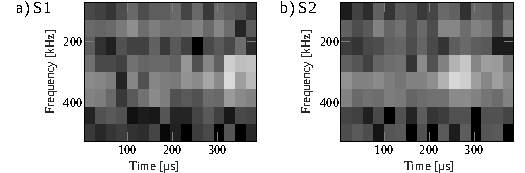
\includegraphics[width=\columnwidth]{../figures/histograms/spectrograms.pdf}
	\caption{Spectrograms of sensors $S_1, S_2$ converted to grayscale for pulses at $x =0.105$, $y = 0.109$ with noise disturbance.}
	\label{fig:spectrograms}
\end{figure}

\begin{figure}[t!]
	\centering
	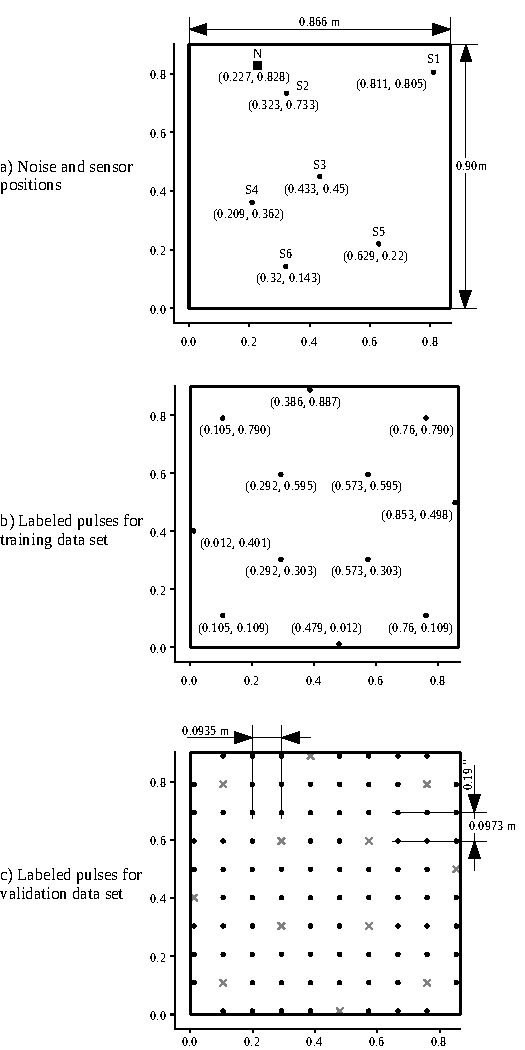
\includegraphics[width=\columnwidth]{../figures/histograms/data_set.pdf}
	\caption{Experimental setup for sensor analytics on structural health monitoring.}
	\label{fig:data_set}
\end{figure}

\subsubsection{CNN-Regression Model}
The data analytics is implemented with a CNN-regression model, see \fig{fig:model}. The structure of the model is described below:

\begin{enumerate}[label=\alph*)]
\item Input tensor. This is composed of spectrograms from the sensor signals. The tensor shape is defined by $S \times T \times F$, where $S$ is the number of sensors, and $T \times F$ is the time-frequency resolution of the spectrograms, see \fig{fig:model}(a).

\item Feature extraction. This is composed of three blocks of convolution, batch normalization, and max-pooling layers, see \fig{fig:model}(b). The number of channels in the convolution layers are defined by the hyper-parameters $A$, $B$, and $C$.

\item Regression function. This is an arbitrary function implemented with two fully connected layers and an output layer with linear activation, see \fig{fig:model}(c).
\end{enumerate}


\begin{figure}[t!]
	\centering
	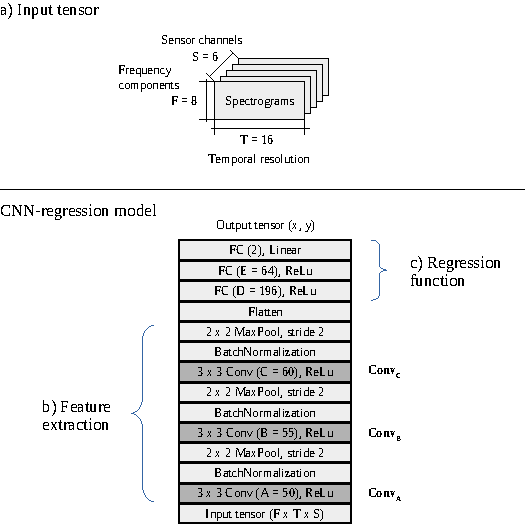
\includegraphics[width=\columnwidth]{../figures/models.pdf}
	\caption{CNN-regression model for sensor analytics.}
	\label{fig:model}
\end{figure}


\subsection{Training}
\subsubsection{Base Model}
The model in \fig{fig:model} is trained using Adam algorithm with iterative early stop, described in \Algo{alg:training}. The Adam optimizer is configured with the default settings presented in \cite{kingma2014adam}: $\alpha = 0.001$, $\beta_1 = 0.9$, $\beta_2 = 0.999$, and $\epsilon = 1\mathrm{e}{-8}$. The training cycle patience is 10 iterations, the optimizer is executed with early stop patience of 10 epochs, and mini-batch size of 512 samples. ($N_I = 10$, $N_E=10$, $B_{size}=512$.)

The training results are illustrated in \fig{fig:optimization}(a). The initial model is obtained at the first early stop. Each stop initializes the moving averages of the Adam optimizer. In subsequent iterations, the model gets updated when the optimizer reaches a better minimum.

\begin{figure}[h!]
	\centering
	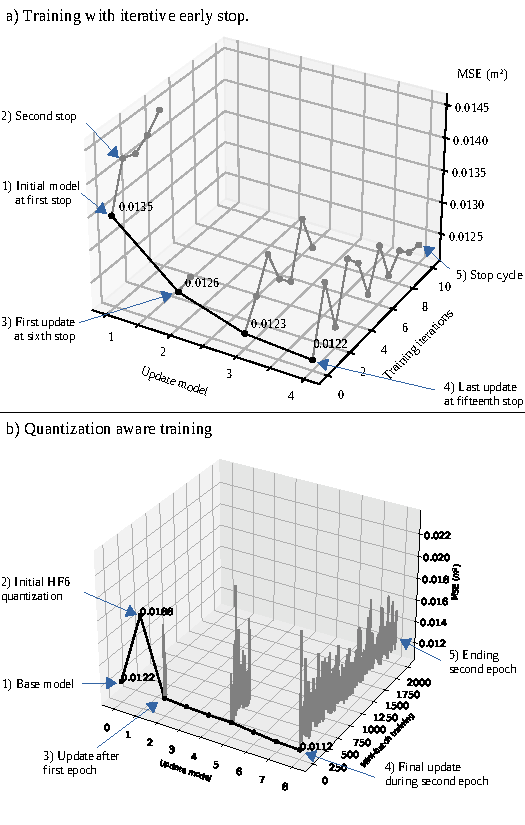
\includegraphics[width=\columnwidth]{../figures/histograms/training_and_quantization.pdf}
	\caption{Training results.}
	\label{fig:optimization}
\end{figure}

The resulting model achieves $MSE=0.0122m^2$ and $MAE=0.0955m$. See \fig{fig:model_evaluation}(a). In total, the training takes 379 epochs in 25 stops. The first stop takes 43 epochs for the initial model and subsequent training iterations take an average of 14 epochs. The training time is 53 minutes using a PC with AMD Ryzen 5 5600H and NVIDIA GeForce RTX 3050.

\begin{figure}[h!]
	\centering
	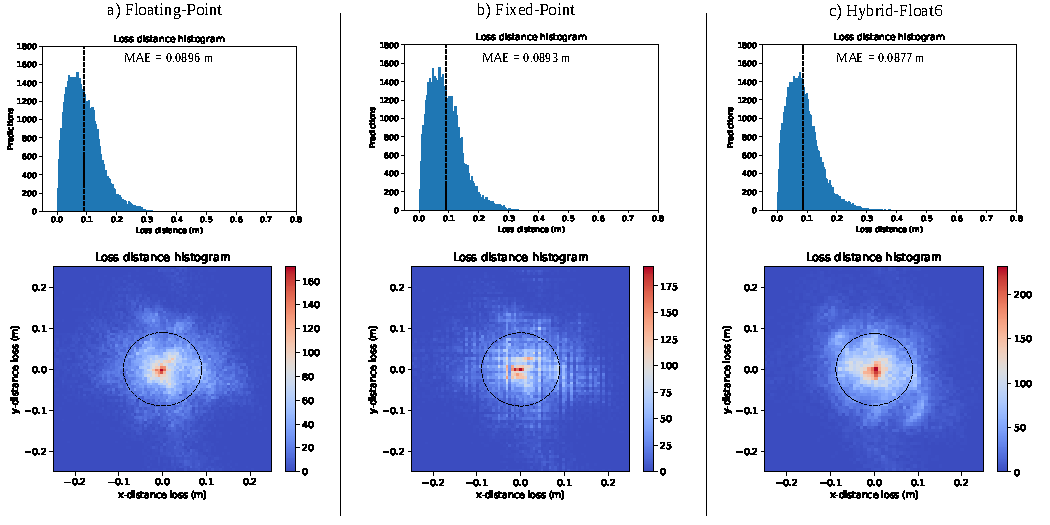
\includegraphics[width=\columnwidth]{../figures/histograms/model_evaluation.pdf}
	\caption{Performance of the model with different data representations.}
	\label{fig:model_evaluation}
\end{figure}

\subsubsection{TensorFlow Lite 8-bit quantization}
This integer quantization is an optimization method that converts 32-bit floating-point numbers (such as weights and activations) to the nearest 8-bit fixed-point numbers. This quantization scheme allows inference to be carried out using integer-only arithmetic\cite{hannwindowsine}.

The base model is quantized using the TensorFlow Lite library with integer-only quantization settings. The filter and bias tensors are represented by 8-bit and 32-bit signed integers, respectively. The input and output activation tensors are represented by 8-bit signed integer. For convolution layers, this quantization includes two additional tensor coefficients (output-multiplier and output-shift). These tensors are the same shape as the bias tensor and are represented by 32-bit signed integers.

The fixed-point model achieves $MSE=0.0122 m^2$ and $MAE=0.0952m$. See \fig{fig:model_evaluation}(b). The MAE gets a reduction of 0.31\% compared to the base model. We attribute this to the regularization effect.

\subsubsection{Quantization Aware Training for Hybrid-Float6}
The QAT is a post-training step, this is applied with the method described in \Algo{alg:quantization_integration}. We run this method during two epochs with mini-batch size of 10 samples with 4-bit exponent and 1-bit mantissa as parameters. ($N_{ep}=2$, $B_{size}=10$, $E_{size}=4$, $M_{size}=1$.)

The QAT is illustrated in \fig{fig:optimization}(b). Initially, the model is quantized with HF6 format (without QAT), this obtains $MSE=0.0188m^2$ and $MAE=0.1232m$. This represents the inference of the base model without QAT on HF6 hardware. See \fig{fig:model_evaluation}(c). The final model after QAT achieves $MSE=0.0112$ and $MAE=0.0919$, these correspond to 8.2\% and 3.77\% error reduction, respectively. See \fig{fig:model_evaluation}(d). The QAT time is 185 minutes.

\subsubsection{Quantization Aware Training for Hybrid-Logarithmic 6-bit}
To compare the inference with 6-bit logarithmic quantization, we execute the QAT on the base model with hybrid-logarithmic parameters. The filter and bias tensors of convolution layers are represented by 6-bit signed logarithmic. The input and output activation tensors are represented by standard floating-point. This is applied with \Algo{alg:quantization_integration}. ($N_{ep}=2$, $B_{size}=10$, $E_{size}=5$, $M_{size}=0$.)

The model achieves $MSE=0.0123$ and $MAE=0.0968$, which correspond to 0.82\% and 1.36\% error increase, respectively. See \fig{fig:model_evaluation}(e).

A summary of the inference with different data representations is presented in \fig{fig:model_evaluation}(f).

\subsection{Hardware Design Exploration}
The proposed hardware/software co-design is demonstrated on the Zynq-7007S system-on-chip (SoC) on the MiniZed development board. This SoC integrates a single ARM Cortex-A9 processing system (PS) and programmable logic (PL) equivalent to Xilinx Artix-7 (FPGA) in a single chip \cite{xilinx2015zynq}. The Zynq-7007S SoC architecture maps the custom logic and software in the PL and PS, respectively.

In this platform, we implement the proposed hardware/software architecture to deploy the sensor analytics application. The desired model is converted to TensorFlow Lite (floating-point) and deployed on the MiniZed. The 6-bit floating-point representation is extracted from the standard floating-point in the HF6 hardware. The Zynq-7007S SoC performs inference executing TensorFlow Lite on the PS. The computational workload of convolution layers is delegated to the dedicated hardware.

\subsubsection{Benchmark on Embedded CPU}
We examine the performance of the embedded CPU for inference without dedicated hardware acceleration. In this case, TensorFlow Lite builds the CNN as a sequential model mapping the entire computation to the CPU (ARM Cortex-A9) at 666 MHz and a power dissipation of $1.187W$.

The compute performance and inference schedule of the model on the CPU is shown in \Tab{tab:performance}(a) and \fig{fig:runtime}(a), respectively.

\subsubsection{Benchmark on Tensor Processor with Standard Floating-Point Hardware}
For this design, we implement the TP with standard floating-point hardware. The design parameters are:
\begin{itemize}
	\item Max convolution kernel size: $K_W = K_H = 3$.
	\item Max input tensor width: $W_I = 16$.
	\item Max input and output channels: $C_I = 55$, $C_O = 60$.
	\item Filter and bias bit-size: $BitSize_F=BitSize_B=32$.
	\item Input tensor bit-size: $BitSize_I=32$.
\end{itemize}

Using equations from Section \ref{sec:memory_utilization}, the on-chip memory requirements are $Input_M=84,480b$, $Filter_M=950,400b$, $Bias_M=1,920b$. Hence, the required on-chip memory buffer size is $TP_B=1,036,800b$.

The post-implementation resource utilization and power dissipation are presented in \Tab{tab:resource_utilization}(a). The complete hardware platform utilizes 83\% of BRAM, this includes the on-chip memory requirements of the TP, DMA, and AXI interconnects. The total available on-chip memory (BRAM) on the Zynq-7007S SoC is 1.8Mb. The estimated power dissipation of the TP is $85mW$ at $200MHz$ (this estimation is provided by Xilinx Vivado).

\begin{table}[!htp]\centering
	\caption{Resource utilization and power dissipation on the Zynq-7007S SoC.}\label{tab:resource_utilization}
	\scriptsize
	\begin{tabular}{lrrrrrr}\toprule
		\multirow{2}{*}{\textbf{TP engine}} &\multicolumn{4}{c}{\textbf{Post-implementation resource utilization}} &\multirow{2}{*}{\textbf{Power (W)}} \\\cmidrule{2-5}
		&\textbf{LUT} &\textbf{FF} &\textbf{DSP} &\textbf{BRAM 36Kb} & \\\midrule
		\multirow{2}{*}{(a) Floating-Point} &5,578 &8,942 &23 &41.5 &\multirow{2}{*}{1.429} \\
		&39\% &31\% &35\% &\textbf{83\%} & \\
		\multirow{2}{*}{(b) Hybrid-Float6} &7,313 &10,330 &20 &15 &\multirow{2}{*}{1.424} \\
		&51\% &36\% &30\% &\textbf{30\%} & \\
		\bottomrule
	\end{tabular}
\end{table}

The compute performance and inference schedule of the model on this hardware implementation is shown in \Tab{tab:performance}(b) and \fig{fig:runtime}(b), respectively. In this implementation, TensorFlow Lite delegates computation of \emph{Conv2D} tensor operations to the TP.

The implementation of dot-product with standard floating-point arithmetic (IEEE 754) utilizes proprietary multiplier and adder floating-point operator cores. Vivado HLS implements floating-point arithmetic operations by mapping them onto Xilinx LogiCORE IP cores, these floating-point operator cores are instantiated in the resultant RTL \cite{hrica2012floating}. In this case, the implementation of the dot-product with the standard floating-point computation reuses the multiplier and adder cores already instantiated in other compute sections of the TP. The post-implementation resource utilization and power dissipation of the floating-point operator cores are shown in \Tab{tab:LogiCORE}.

\begin{table}[!htp]\centering
	\caption{Compute performance of the CPU and TP on each Conv2D tensor operation. This table presents: tensor operation, computational cost, latency, throughput, power efficiency, and estimated energy consumption.}\label{tab:performance}
	\scriptsize
	\begin{tabular}{lrrrrrr}\toprule
		\textbf{Operation} &\textbf{MFLOP} &\textbf{t (ms)} &\textbf{MFLOP/s} &\textbf{MFLOP/s/W} &\textbf{EDP (mJ)} \\\midrule
		& &\multicolumn{4}{l}{\textbf{a) CPU @666MHz, 1.187 W}} \\
		Conv\textsubscript{A} &0.691 &112.24 &6.16 &5.19 &133.23 \\
		Conv\textsubscript{B} &1.584 &213.13 &7.43 &6.26 &252.99 \\
		Conv\textsubscript{C} &0.475 &46.59 &10.20 &8.59 &55.31 \\
		& &\multicolumn{4}{l}{\textbf{b) TP Floating-Point @200MHz, 85 mW}} \\
		Conv\textsubscript{A} &0.691 &12.49 &55.34 &651.11 &1.06 \\
		Conv\textsubscript{B} &1.584 &16.39 &96.66 &1,137.20 &1.39 \\
		Conv\textsubscript{C} &0.475 &3.59 &132.44 &1,558.13 &0.30 \\
		& &\multicolumn{4}{l}{\textbf{c) TP Hybrid-Float6 @200MHz, 84 mW}} \\
		Conv\textsubscript{A} &0.691 &6.92 &99.81 &1,188.24 &0.58 \\
		Conv\textsubscript{B} &1.584 &4.41 &358.94 &4,273.09 &0.37 \\
		Conv\textsubscript{C} &0.475 &0.99 &482.44 &5,743.29 &0.08 \\
		\bottomrule
	\end{tabular}
\end{table}


\begin{table}[!h]\centering
	\caption{Resource utilization and power dissipation of multiplier and adder floating-point (IEEE 754) operator cores (Xilinx LogiCORE IP).}\label{tab:LogiCORE}
	\scriptsize
	\begin{tabular}{lrrrrrr}\toprule
		\textbf{Core operation} &\textbf{DSP} &\textbf{FF} &\textbf{LUT} &\textbf{Latency (clk)} &\textbf{Power (mW)} \\\midrule
		Multiplier &3 &151 &325 &4 &7 \\
		Adder &2 &324 &424 &8 &6 \\
		\bottomrule
	\end{tabular}
\end{table}



\subsubsection{Tensor Processor with Hybrid-Float6 Hardware}
For the proposed design, the TP with HF6 hardware restates the standard floating-point design with the following customization: $BitSize_F=BitSize_B=6$.

Using equations from Section \ref{sec:memory_utilization}, the on-chip memory requirements are $Input_M=84,480b$, $Filter_M=178,200b$, $Bias_M=360b$. Hence, the required on-chip memory buffer size is $TP_B=263,040b$.

The post-implementation resource utilization and power dissipation are presented in \Tab{tab:resource_utilization}(b). The complete hardware platform utilizes 30\% of BRAM, this includes the on-chip memory requirements of the TP, DMA, and AXI interconnects. The estimated power dissipation of the TP is $84mW$ at $200MHz$ (this estimation is provided by Xilinx Vivado).

The compute performance and inference schedule of the model on this hardware implementation is shown in \Tab{tab:performance}(c) and \fig{fig:runtime}(c), respectively.

\begin{figure}[t!]
	\centering
	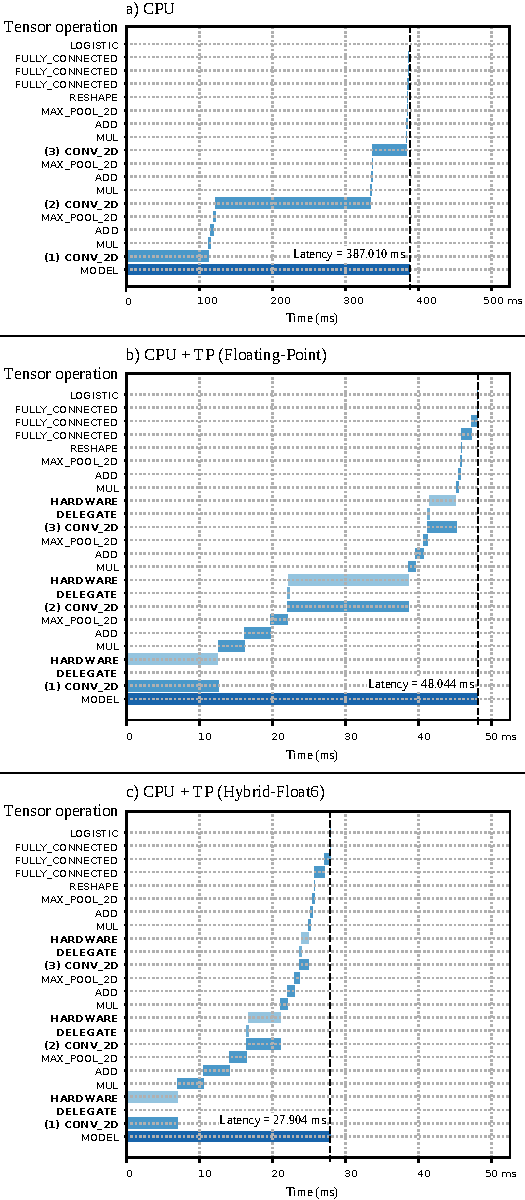
\includegraphics[width=1\columnwidth]{../figures/runtime/runtime.pdf}
	\caption{Run-time inference of TensorFlow Lite on the Zynq-7007S SoC. (a) CPU ARM Cortex-A9 at 666MHz, (b) cooperative CPU + TP with floating-point Xilinx LogiCORE IP at 200MHz, and (c) cooperative CPU + TP with Hybrid-Float6 at 200MHz.}
	\label{fig:runtime}
\end{figure}

\subsection{Results and discussion}
\subsubsection{Training}
The TensorFlow Lite 8-bit quantization preserves accuracy of the model. The regularization effect in this quantization can benefit the solution. However, the error distribution in linear regressions gets highly discretized. The HF6 quantization qualitatively improves the error distribution and the accuracy of the model. See \fig{fig:2d_error_distribtion}.

\begin{figure}[t!]
	\centering
	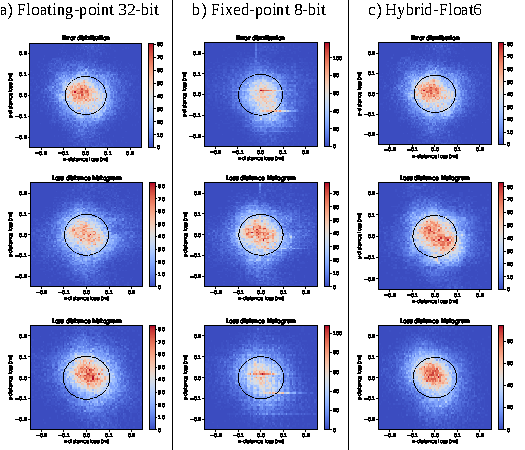
\includegraphics[width=1\columnwidth]{../figures/histograms/2D_error_distribtion.pdf}
	\caption{2D error distribution of the CNN-regression model.}
	\label{fig:2d_error_distribtion}
\end{figure}

The hybrid dot-product with custom floating-point does not reuse the available floating-point operator cores instantiated from other computational sections (see {\Tab{tab:LogiCORE}}). Therefore, the logic required for the dot-product must be implemented, which is reflected as additional utilization of LUT and FF resources.


\begin{figure}[t!]
	\centering
	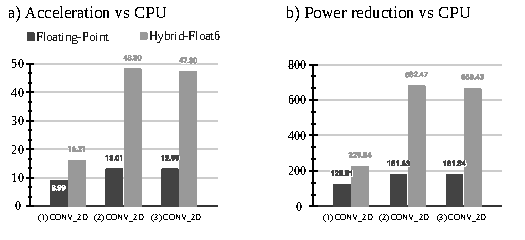
\includegraphics[width=1\columnwidth]{../figures/power_breakdown/acceleration_power_reduction.pdf}
	\caption{Inference acceleration and power reduction on the TP with floating-point and HF6 vs. CPU on the Zynq-7007S SoC.}
	\label{fig:acceleration}
\end{figure}

\begin{figure}[t!]
	\centering
	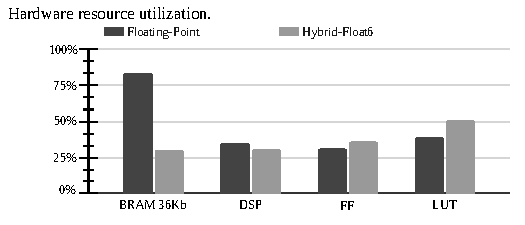
\includegraphics[width=1\columnwidth]{../figures/power_breakdown/resource_utilization.pdf}
	\caption{Hardware resource utilization on the Zynq-7007S SoC.}
	\label{fig:resource_utilization}
\end{figure}

\begin{figure}[t!]
	\centering
	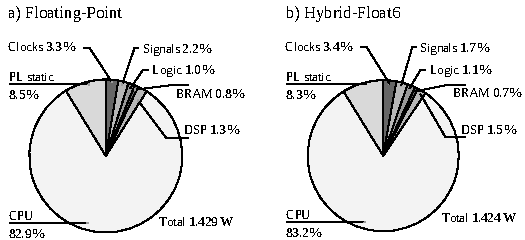
\includegraphics[width=1\columnwidth]{../figures/power_breakdown/power_breakdown.pdf}
	\caption{Estimated power dissipation on the Zynq-7007S SoC with PS at 666MHz and PL at 200MHz.}
	\label{fig:power}
\end{figure}